\Annex{Annexe des architectures d'assistants conversationnels (\textit{chatbot})}
\label{annex:B-ANNEXE-CHATBOT}
	
	% INTRODUCTION DE L'ANNEXE.
	
	% Engoument pour les chatbots en 2019.
	Au début de ce doctorat (\texttt{octobre 2019}), on pouvait noter que :
	\begin{itemize}
		\item selon \cite{costello-lodolce:2019:gartner-top-technologies}, \textguillemets{seuls $4$\% des clients de \texttt{Gartner} [déclaraient] utiliser des \textit{chatbot} sur leur lieu de travail, mais $40$\% [avaient] l'intention de les mettre en oeuvre à court terme} ;
		\item et selon \cite{goasduff:2019:chatbots-will-appeal}, \textguillemets{d'ici 2022, 70\% des employés [interagiraient] quotidiennement avec les plateformes conversationnelles}.
	\end{itemize}
	
	% Engoument pour les chatbots en 2023.
	Aujourd'hui (\texttt{octobre 2023}), le mot \textit{chatbot} est sur toutes les lèvres, surtout depuis la révolution des \texttt{IA} génératives lancées par \texttt{ChatGPT} (\cite{openai:2023:chatgpt}) :
	\begin{itemize}
		\item selon \cite{costello-lodolce:2022:gartner-predicts-chatbots}, une entreprise sur deux aurait actuellement recours à une forme de \textit{chatbot} pour gérer sa relation client, et \textguillemets{d'ici 2027, les \textit{chatbot} deviendront le principal canal de service client pour environ un quart des organisations}.
	\end{itemize}

	% Annonce du plan.
	Dans cette annexe, nous allons détailler brièvement les philosophies de conceptions d'assistants conversationnels.
	
	% Citation.
	\begin{leftBarInformation}
		Cette présentation s'inspire des articles de \cite{chen-etal:2017:survey-dialogue-systems} et de \cite{adamopoulou-moussiades:2020:overview-chatbot-technology}.
	\end{leftBarInformation}
	
	% TABLE DES MATIÈRES DE L'ANNEXE.
	\minitoc
	
	
	% Exemple de projet task-oriented: \cite{yan-etal:2017:building-taskoriented-dialogue}
	
	% \cite{brabra-etal:2022:dialogue-management-conversational}: plusieurs système de gestion du dialogue : soit implémenté manuellement, soit entraîné, soit hybride.
	
	% Note auteur: une confusion fréquente est "task-based" => "not deep-learning"
	
	% % Introduction: classification des \textit{chatbots} en .
	\todo[inline]{A REDIGER}
	D'après \cite{chen-etal:2017:survey-dialogue-systems} et \cite{adamopoulou-moussiades:2020:overview-chatbot-technology}, nous pouvons distinguer grossièrement les \textit{chatbots} en deux approches en fonction de leur objectif principal :
	\begin{itemize}
		\item d'une part, il y a les \textit{chatbots} \textguillemets{\textit{task-oriented}}, axés sur l'accomplissement d'une tâche précise ;
		\item d'autre part, il y a les \textit{chatbots} \textguillemets{\textit{chat-oriented}}, dont l'utilité première est basée sur leur capacité à entretenir une conversation avec l'utilisateur.
	\end{itemize}
	
	La \textsc{Figure~\ref{figure:B.2-CHATBOT-ARCHITECTURES}} représente ces deux approches par leurs architectures les plus communes.
	\begin{figure}[!htb]
		\centering
		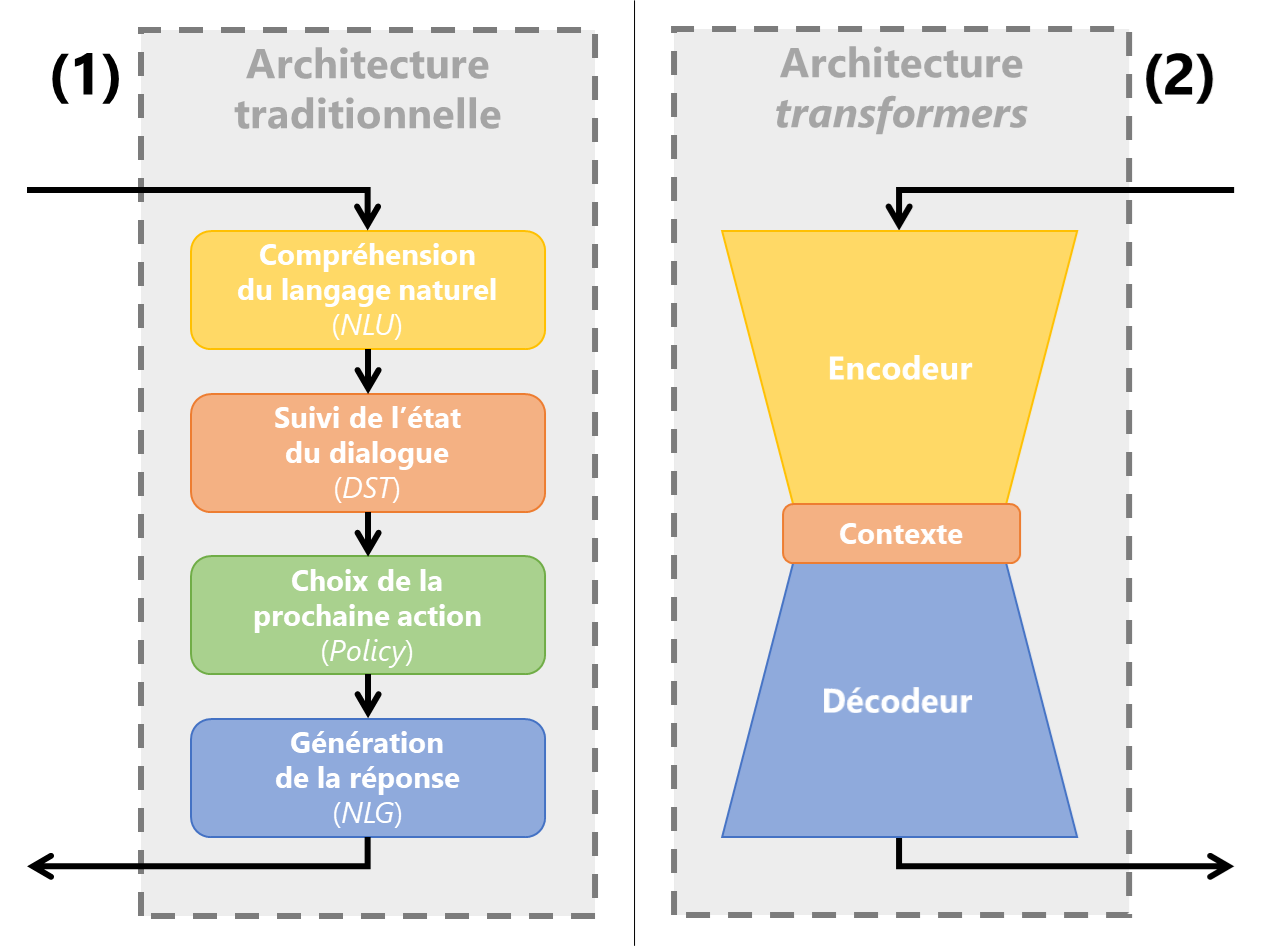
\includegraphics[width=0.95\textwidth]{figures/annexe-chatbots-architectures}
		\caption{
			Schéma illustrant les deux architecture usuelles pour implémenter un assistant conversationnel :
			\textbf{(1)} représente les \textbf{approches symboliques} avec un schéma d'architecture de gestion d'états de dialogue,
			et \textbf{(2)} représente les \textbf{approches génératives} avec un schéma d'architecture à base de \textit{transformers}, composée d'un encodeur et d'un décodeur.
		}
		\label{figure:B.2-CHATBOT-ARCHITECTURES}
	\end{figure}
	
	
	%%%%%--------------------------------------------------------------------
	%%%%% Annexe B.1: Classification des \textit{chatbots} suivant leurs objectifs.
	%%%%%--------------------------------------------------------------------

		% \subsection{Les \textit{chatbots} \textguillemets{\textit{task-oriented}}}
		% \label{annex:B.1.1-CHATBOT-CLASSIFICATION-TASK-ORIENTED}
		
			% % Définition.
				% Un \textit{chatbot} \textguillemets{\textit{task-oriented}} est conçu pour \textbf{accomplir une tâche spécifique}.
				% Le parcours de dialogue proposé est généralement prédéfini et comporte peu de digressions : l'assistant détermine l'action à réaliser grâce à l'énoncé de l'utilisateur, demande éventuellement des compléments d'informations si la requête n'est pas assez précise, puis effectue sa mission.
				% Le périmètre de fonctionnalités est généralement restreint pour contrôler les actions de l'assistant et s'assurer de son comportement.
			
			% % Exemples de fonctionnalités.
				% Gérer la relation client (\textit{suivi de commande, formulaire de satisfaction, ...}) ;
				% Accéder à des informations documentaires ou personnelles (\textit{accès à une documentation technique, accès au solde d'un compte bancaire, ...}) ;
				% Pré-remplir d'un formulaire (\textit{réserver un billet de voyage, payer ses contraventions, faire opposition à sa carte de crédit, ...}) ;
				 % Gérer la domotique (\textit{allume la lumière, joue de la musique, active l'alarme, ...}).
			
			% % Exemples d'assistants conversationnels connus.
				% \texttt{Assistant Virtuel SNCF} (\cite{sncf:2018:agent-virtuel-sncf}) pour la réservation de billets de train ;
				% \texttt{Google Assistant} (\cite{google:2016:google-assistant-your}) et \texttt{Alexa} (\cite{alexa-internet:2018:keyword-research-competitor}) pour la gestion de la domotique.
		
		
		% \subsection{Les \textit{chatbots} \textguillemets{\textit{chat-oriented}}}
		% \label{annex:B.1.2-CHATBOT-CLASSIFICATION-CHAT-ORIENTED}
		
			% % Définition.
				% Un \textit{chatbot} \textguillemets{\textit{chat-oriented}} se concentre davantage sur les interactions avec l'utilisateur dans le but d'\textbf{engager la conversation}.
				% Son objectif principale est de rendre le dialogue agréable.
				% Son périmètre de connaissance n'est en général pas restreint pour pouvoir facilement engager la conversation sur n'importe quel sujet.
		
			% % Exemples de fonctionnalités.
				% Offrir du divertissement (\textit{raconter une histoire ou une blague, organiser un jeu narratif, ...}) ;
				% Proposer une assistance générale (\textit{donner une définition, demander une explication, ...}) ;
				% Simplement discuter (\textit{mimer les interactions sociales}).
			
			% % Exemples d'assistants conversationnels connus.
				% \texttt{ELIZA} (\cite{weizenbaum:1966:eliza-computer-program}) pour simuler un entretien clinique en psychothérapie ;
				% \texttt{AI Dungeon} (\cite{latitude-inc.-oasis-tech-inc.:2019:ai-dungeon}) pour participer à la narration d'histoires interactives ;
				% \texttt{ChatGPT} (\cite{openai:2023:chatgpt}) et \texttt{BARD} (\cite{google:2023:bard-chat-based}) pour discuter avec des larges modèles de langues (\texttt{LLM}).
	
	
	%%%%--------------------------------------------------------------------
	%%%% Annexe B.2: Architectures usuelles des chatbots.
	%%%%--------------------------------------------------------------------
	% \section{Architectures usuelles des chatbots}
	% \label{annex:B.2-CHATBOT-ARCHITECTURES}

		% % Introduction: classification des \textit{chatbots}.
		% Toujours en s'inspirant de \cite{chen-etal:2017:survey-dialogue-systems} et de \cite{adamopoulou-moussiades:2020:overview-chatbot-technology}, nous pouvons distinguer deux types d'approches principales pour implémenter un \textit{chatbot} :
		% \begin{itemize}
			% \item les \textit{approches symboliques}, traditionnellement utilisées pour traiter le langage en essayant d'en réaliser un modélisation abstraite ;
			% \item les \textit{approches génératives}, reproduisant les capacités du langage en employant les capacités actuelles des réseaux de neurones sur des immenses quantités de données.
		% \end{itemize}
		
		% Ces deux types d'approches sont représentées dans la \textsc{Figure~\ref{figure:B.2-CHATBOT-ARCHITECTURES}}.
		
		% \begin{figure}[!htb]
			% \centering
			% 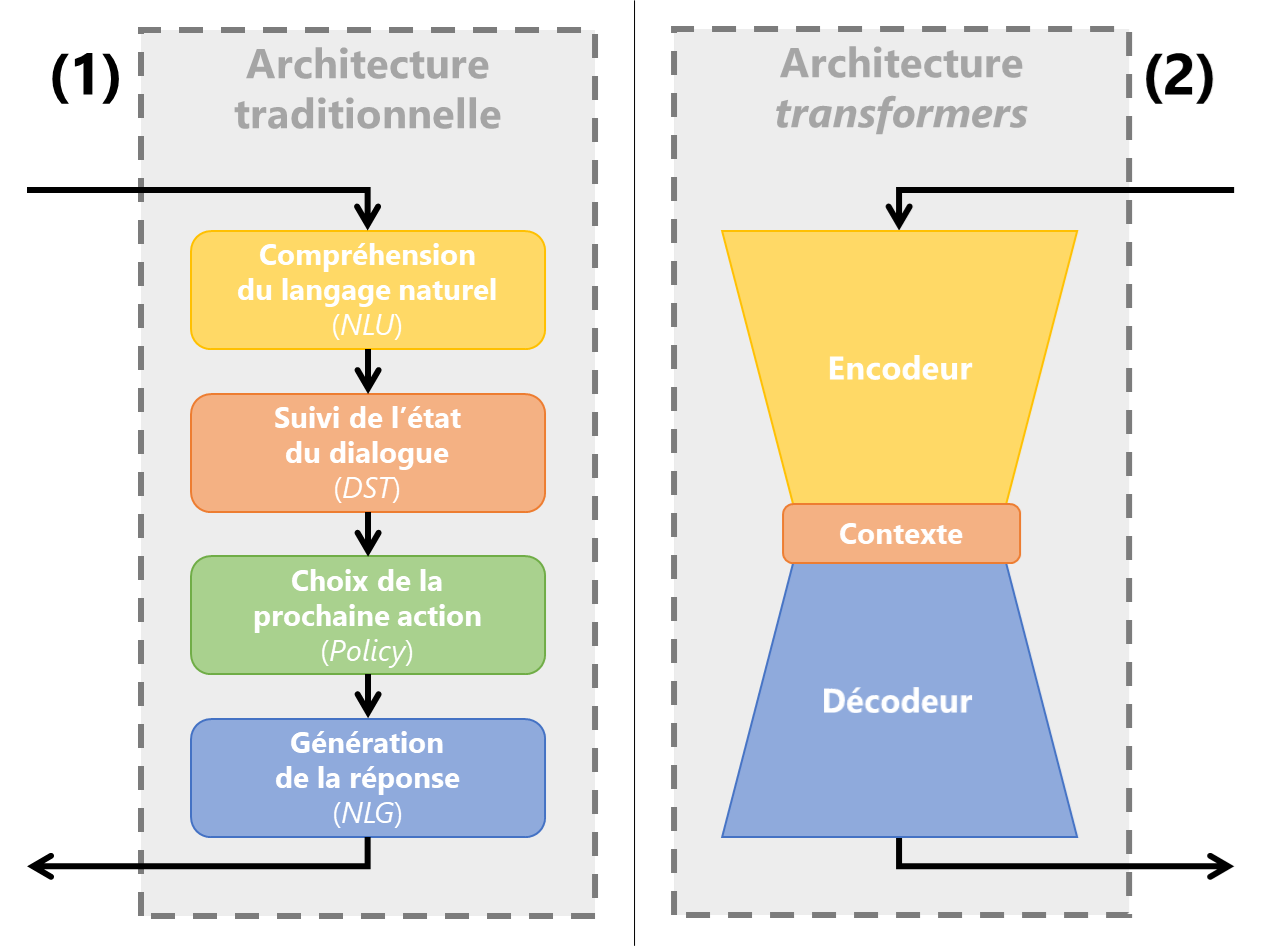
\includegraphics[width=0.95\textwidth]{figures/annexe-chatbots-architectures}
			% \caption{
				% Schéma illustrant les deux architecture usuelles pour implémenter un assistant conversationnel :
				% \textbf{(1)} représente les \textbf{approches symboliques} avec un schéma d'architecture de gestion d'états de dialogue,
				% et \textbf{(2)} représente les \textbf{approches génératives} avec un schéma d'architecture à base de \textit{transformers}, composée d'un encodeur et d'un décodeur.
			% }
			% \label{figure:B.2-CHATBOT-ARCHITECTURES}
		% \end{figure}
		
		
		%%
		%% Subsection B.2.1. Les approches symboliques.
		%%
		% \subsection{Les approches symboliques}
		% \label{annex:B.2.1-CHATBOT-ARCHITECTURES-SYMBOLIQUE}
		% \todo[inline]{A REDIGER}
		
			% % Définition.
			% \paragraph{Définition :}
			
				% \cite{schuurmans-frasincar:2020:intent-classification-dialogue}  \\ % definition intention
			
			% % Exemples d'assistants conversationnels connus.
			% \paragraph{Exemples de moteurs connus ayant une approche symbolique :}
			
				% \texttt{RASA} \cite{bocklisch-etal:2017:rasa-open-source}
				% ou \texttt{WATSON} (\cite{hoyt-etal:2016:ibm-watson-analytics}).
		
		
		%%
		%% Subsection B.2.2. Les approches génératives.
		%%
		% \subsection{Les approches génératives}
		% \label{annex:B.2.2-CHATBOT-ARCHITECTURES-GENERATIVE}
		% \todo[inline]{A REDIGER}
		
			% % Définition.
			% \paragraph{Définition :}
			
				% \cite{uszkoreit:2017:transformer-novel-neural}  \\ % architecture transformers
				% \cite{ni-etal:2022:recent-advances-deep}  \\ % avancer en deep learning
				% \cite{openai:2023:chatgpt}  \\ % exemple
				% \cite{touvron-etal:2023:llama-open-foundation}  \\ % exemple
				% \cite{kaddour-etal:2023:challenges-applications-large} % plusieurs challenges
			
			% % Exemples d'assistants conversationnels connus.
			% \paragraph{Exemples de moteurs connus ayant une approche générative :}
				% \texttt{GPT} (\cite{openai:2023:chatgpt})
				% ou \texttt{LLAMA2} (\cite{touvron-etal:2023:llama-open-foundation}).
	
	
	%%%%--------------------------------------------------------------------
	%%%% Annexe B.3: Discussions sur le niveau d'automatisation.
	%%%%--------------------------------------------------------------------
	% \section{Discussions sur le niveau d'automatisation}
	% \label{annex:B.2-CHATBOT-DISCUSSION-AUTOMATISATION}
		
		% \todo[inline]{A REDIGER}
			
		% \begin{leftBarAuthorOpinion}
			% On amalgame approche générative et chatbot \textit{chat-oriented}.
		% \end{leftBarAuthorOpinion}
		
		% \cite{sheridan-verplank:1978:human-computer-control} repris par \cite{parasuraman-etal:2000:model-types-levels} \\ % 10 niveaux de contrôles